\section{Approche non supervisée par la méthode des k-means}

\textbf{Question 1: Méthode des centres mobiles} \\

L'algorithme des k-moyennes permet de créer des sous-ensembles de données à partir d'un ensemble de base. Pour ce TP, cet
algorithme serait utile pour diviser en clusters les pixels de l'image. \\

\textbf{Question 2: Apprentissage non supervisée du classifieur}

\begin{figure}[!h]
    \begin{minted}[frame=lines, framesep=2mm, baselinestretch=1.2, fontsize=\footnotesize, linenos, breaklines=true]{python}
def unsupervisedTraining(featLearn, method='kmeans'):
    answer = input('nombre de classes:')
    nbCluster = int(answer)
    if method == 'kmeans':
        model = KMeans(n_clusters=nbCluster, random_state=42)
        model.fit(featLearn)
    elif method == 'gmm':
        ...

    return model
    \end{minted}   
    \captionof{listing}{\label{lst:unsupervisedTrainingFunction}UnsupervisedTraining Function}
\end{figure}


Cette fonction est utilisée pour définir le nombre de cluster que l'on veut. Dans notre cas, comme on a pu le voir dans
la partie précédente, on distingue plus ou moins trois clusters de couleur. On indiquera donc que l'on veut trois clusters. \\ 

Les paramètres importants sont le nombre de clusters et les caractéristiques d'entrées dans featLearn.\\

\textbf{Question 3: Prédictions des labels}

\begin{figure}[!h]
    \begin{minted}[frame=lines, framesep=2mm, baselinestretch=1.2, fontsize=\footnotesize, linenos, breaklines=true]{python}
# Apprentissage de la fonction de classement
model = unsupervisedTraining(featLearn, method='kmeans')

# prediction des labels sur la base d'apprentissage
labels_predict = model.predict(featLearn)
    \end{minted}   
    \captionof{listing}{\label{lst:aralseaMain}aralsea Main Function}
\end{figure}

\clearpage

\textbf{Question 4: Visualisation des descripteurs d'apprentissage et de leur classe}

\begin{figure}[!h]
    \begin{minipage}{.48\linewidth}
        \begin{center}
            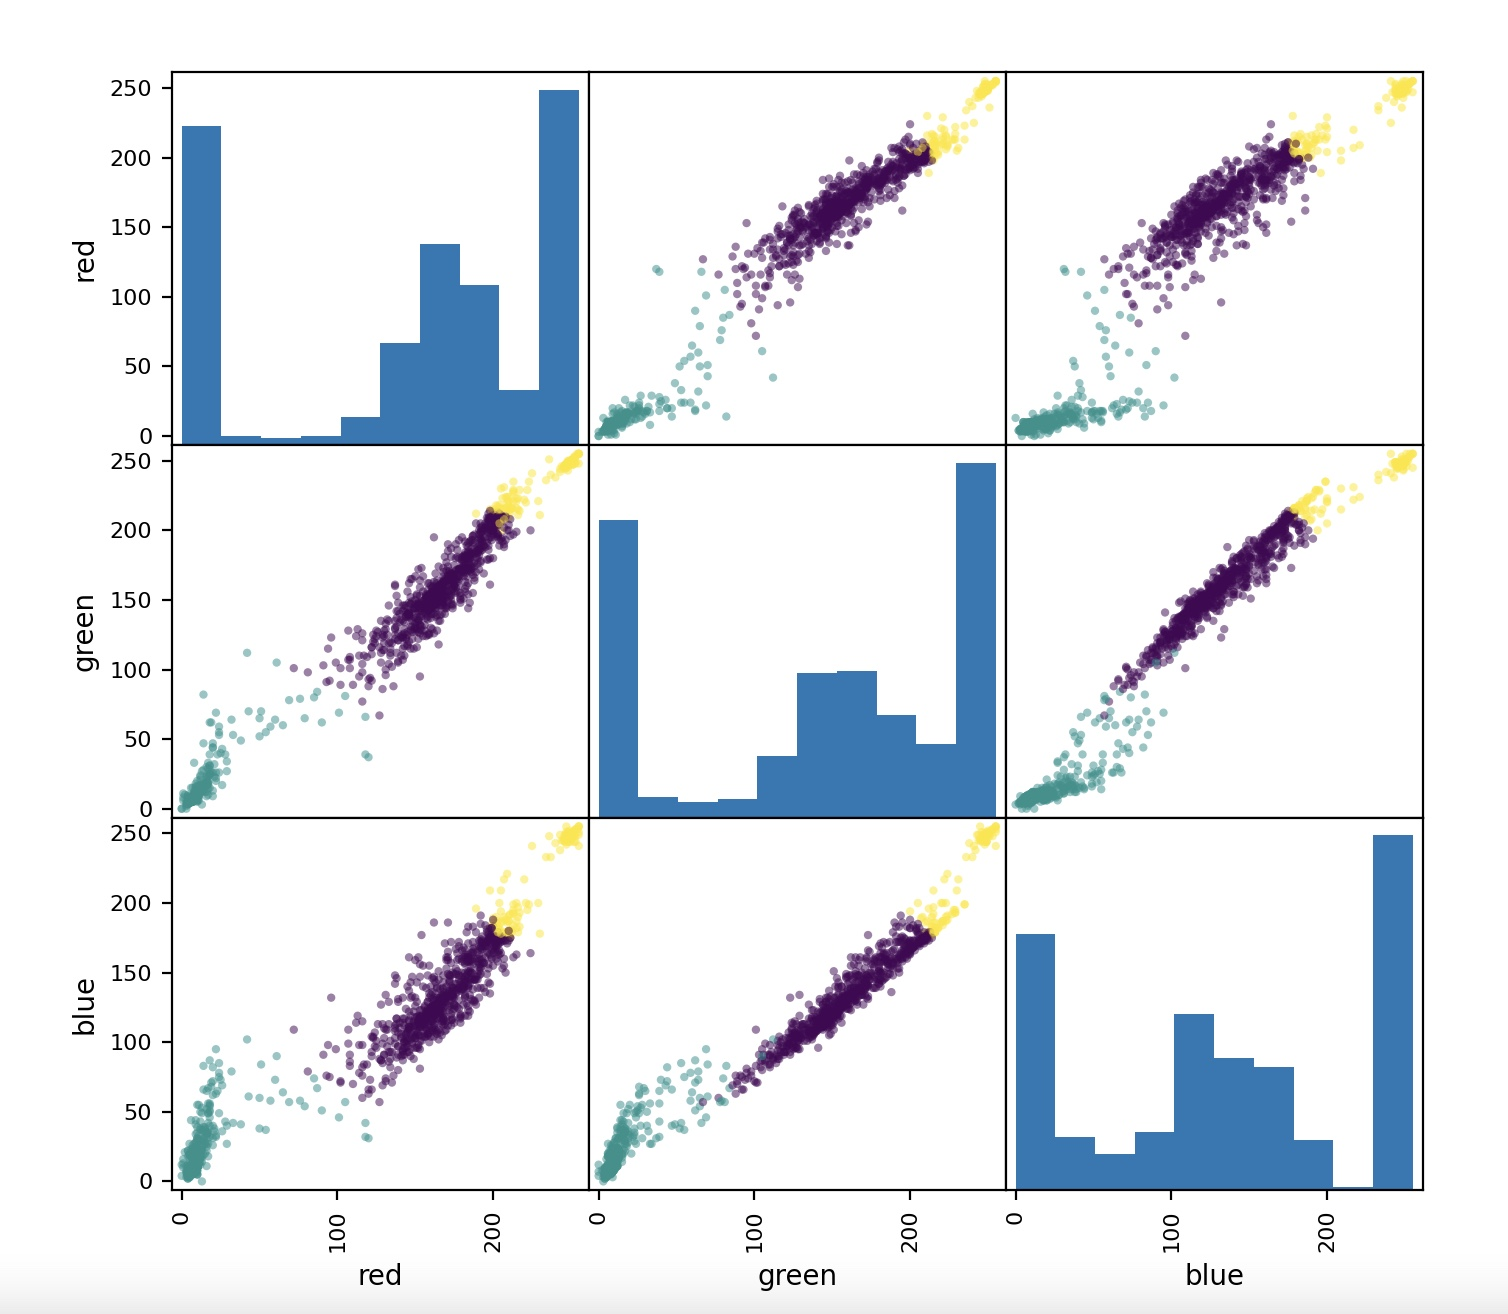
\includegraphics[width=0.75\textwidth]{./img/6.4.1.jpg}
                \caption{\label{fig:6.4.1}Image 2D}  
            \end{center}
    \end{minipage}\hfill
    \begin{minipage}{.48\linewidth}
        \begin{center}
            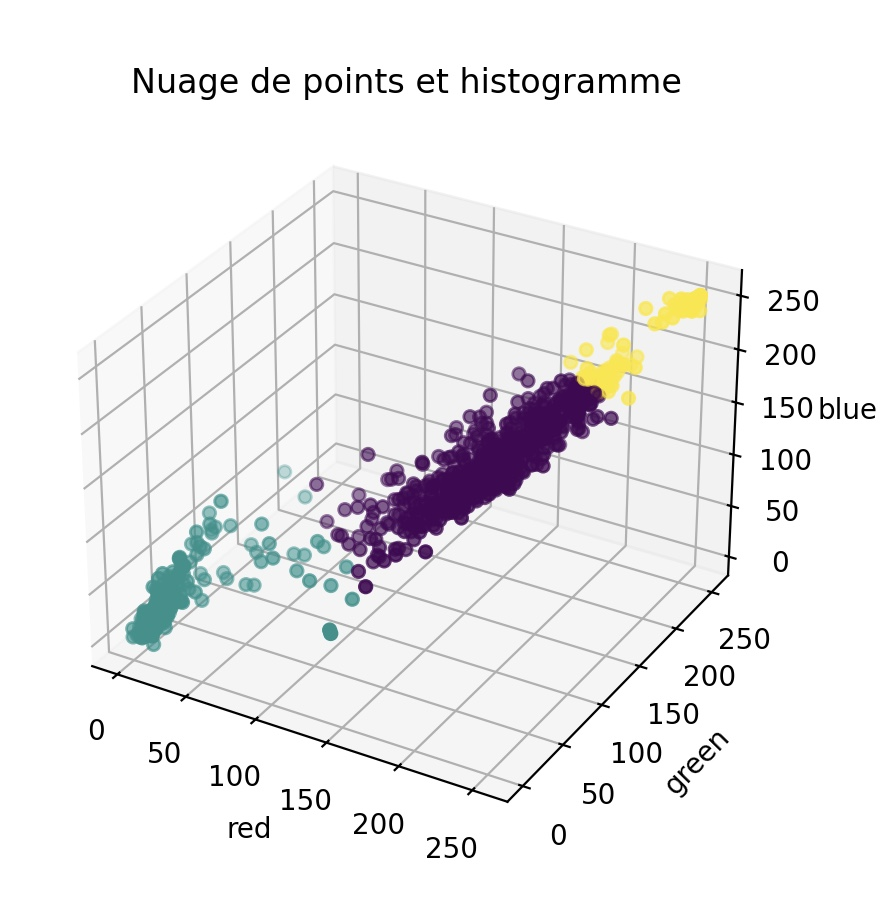
\includegraphics[width=0.75\textwidth]{./img/6.4.2.jpg}
            \caption{\label{fig:6.4.2}Image 3D}  
        \end{center}
    \end{minipage}
\end{figure}

On retrouve sur ces deux graphiques ce que l'on avait prédis à la question.2, on distingue bien trois clusters
de couleurs différents ce qui confirme ce que l'on pensait. \\


\textbf{Question 5: Classification des deux images}

\begin{figure}[!h]
    \begin{minted}[frame=lines, framesep=2mm, baselinestretch=1.2, fontsize=\footnotesize, linenos, breaklines=true]{python}
def unsupervisedClassifying(model, feat):
    height, width, channels = feat.shape
    feat_matrix = feat.reshape((height * width, channels))
    label = model.predict(feat_matrix)

    return label
    \end{minted}   
    \captionof{listing}{\label{lst:unsupervisedClassifyingFunction}unsupervisedClassifying Function}
\end{figure}

\begin{figure}[!h]
    \begin{minted}[frame=lines, framesep=2mm, baselinestretch=1.2, fontsize=\footnotesize, linenos, breaklines=true]{python}
# Classifying / Predicting / Testing
labels_prediction_img73 = unsupervisedClassifying(model, img73)
labels_prediction_img87 = unsupervisedClassifying(model, img87)
    \end{minted}   
    \captionof{listing}{\label{lst:aralsea Function}aralsea Function}
\end{figure}


\textbf{Question 6: Visualisation de la classification des deux images}

\begin{figure}[!h]
    \begin{minipage}{.48\linewidth}
        \begin{center}
            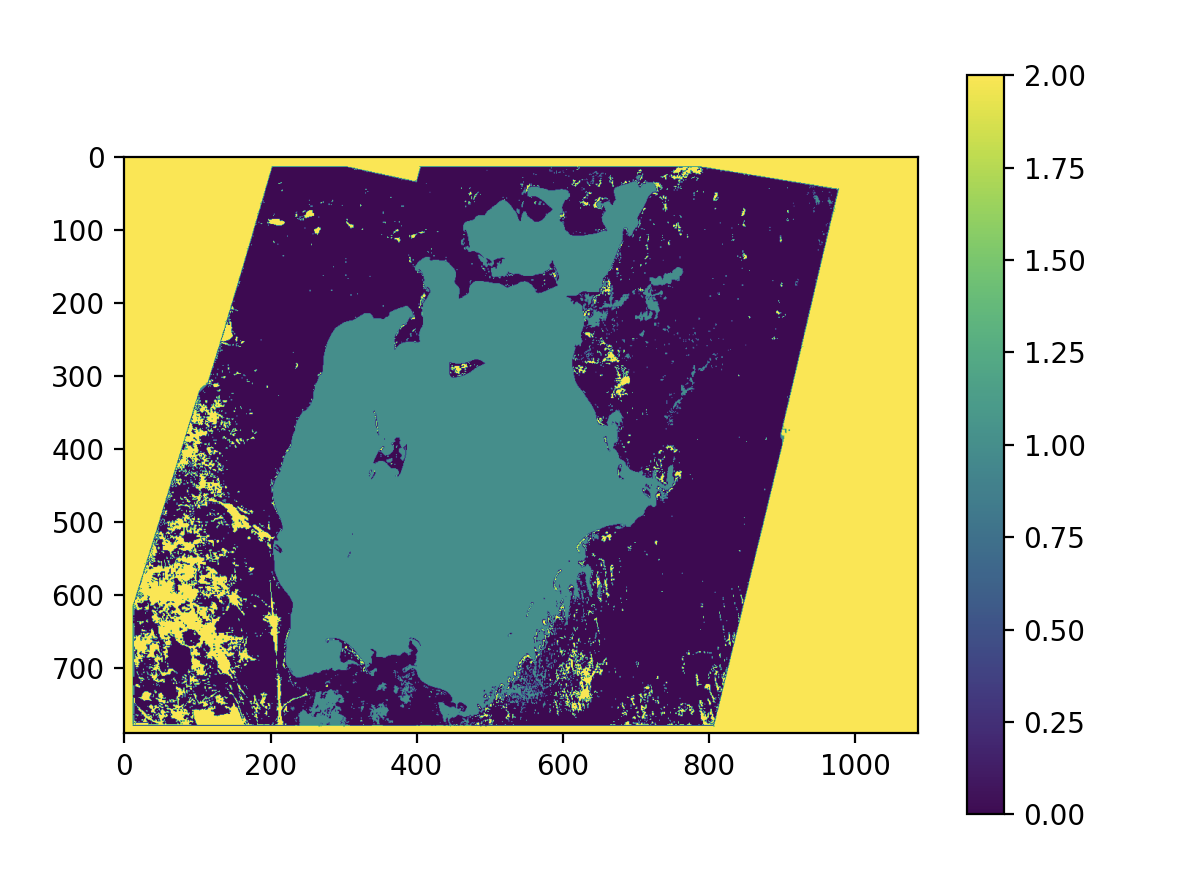
\includegraphics[width=0.75\textwidth]{./img/6.6.1.png}
                \caption{\label{fig:6.4.1}Image 1973 Predicted Labels}  
            \end{center}
    \end{minipage}\hfill
    \begin{minipage}{.48\linewidth}
        \begin{center}
            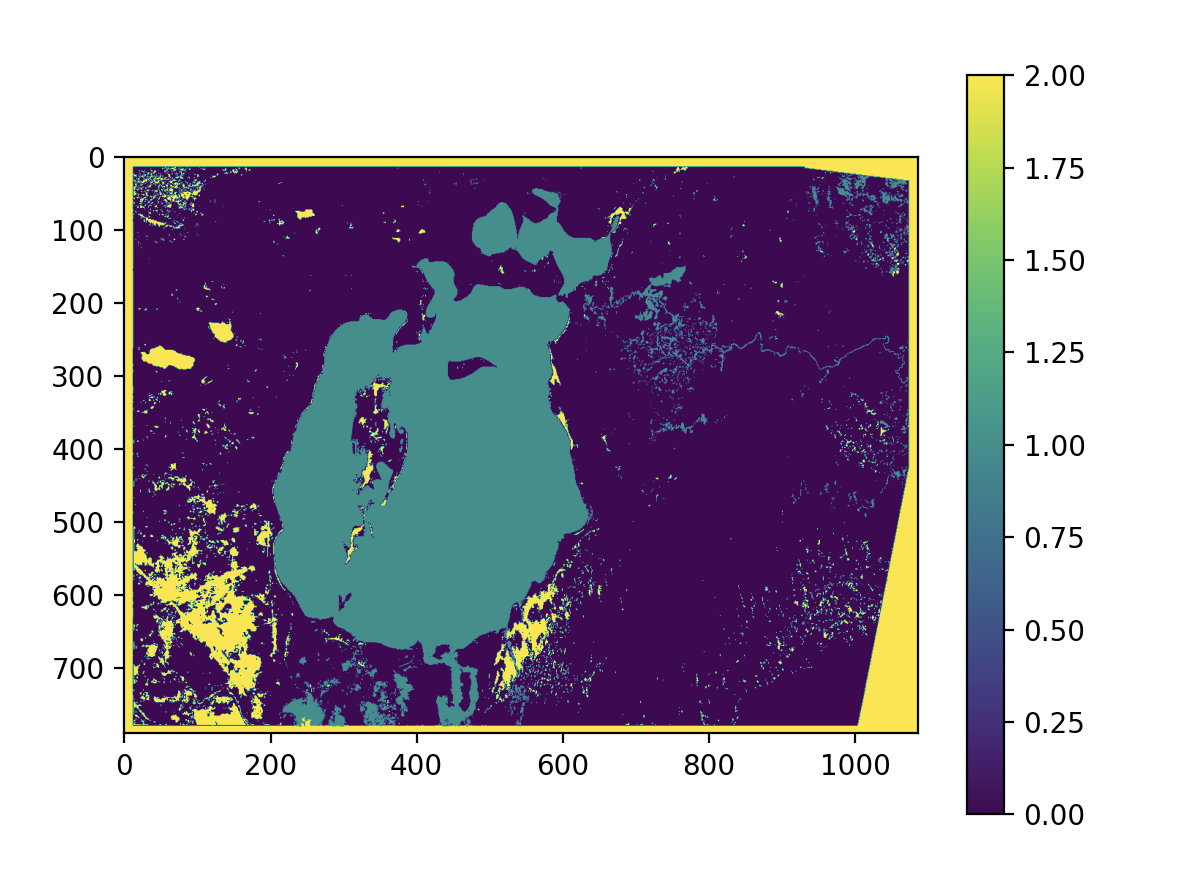
\includegraphics[width=0.75\textwidth]{./img/6.6.2.png}
            \caption{\label{fig:6.4.2}Image 1987 Predicted Labels}  
        \end{center}
    \end{minipage}
\end{figure}

\clearpage

Sur ces deux graphiques, on voit très bien la distinction sur l'image des trois clusters. Sur les deux image, la mer d'Aral est 
visible en vert/cyan, le rivage est visible en très foncé bleu/violet et l'extérieur des images en jaune. \\ 

\textbf{Question 7: Estimation de la surface et de son évolution}

\begin{figure}[!h]
    \begin{minted}[frame=lines, framesep=2mm, baselinestretch=1.2, fontsize=\footnotesize, linenos, breaklines=true]{python}
# Pourcentage de la mer
proportion_mer_img73 = (np.sum(img73_label == 1) / img73_label.size)*100
proportion_mer_img87 = (np.sum(img87_label == 1) / img87_label.size)*100

print("Proportion de la mer dans l'Image 1973:", proportion_mer_img73)
print("Proportion de la mer dans l'Image 1987:", proportion_mer_img87)
print("Une chute du niveau de la mer de:", proportion_mer_img73-proportion_mer_img87)
"""return
Proportion de la mer dans l'Image 1973: 27.632828930016085
Proportion de la mer dans l'Image 1987: 21.373769627030974
Une chute du niveau de la mer de: 6.259059302985111
"""
    \end{minted}   
    \captionof{listing}{\label{lst:aralsea Main Function}SurfaceEvolution Function}
\end{figure}

D'après les résultats obtenus, on a un pourcentage de la mer de 27.63\% en 1973 contre 21.37\% en 1987. L'évolution de la surface
de la mer d'Aral en 14 ans est donc d'approximativement 6.26\%. \\

\textbf{Question 8: Estimation de la surface et de son évolution} \\

\textbf{k=6}

\begin{figure}[!h]
    \begin{minipage}{.48\linewidth}
        \begin{center}
            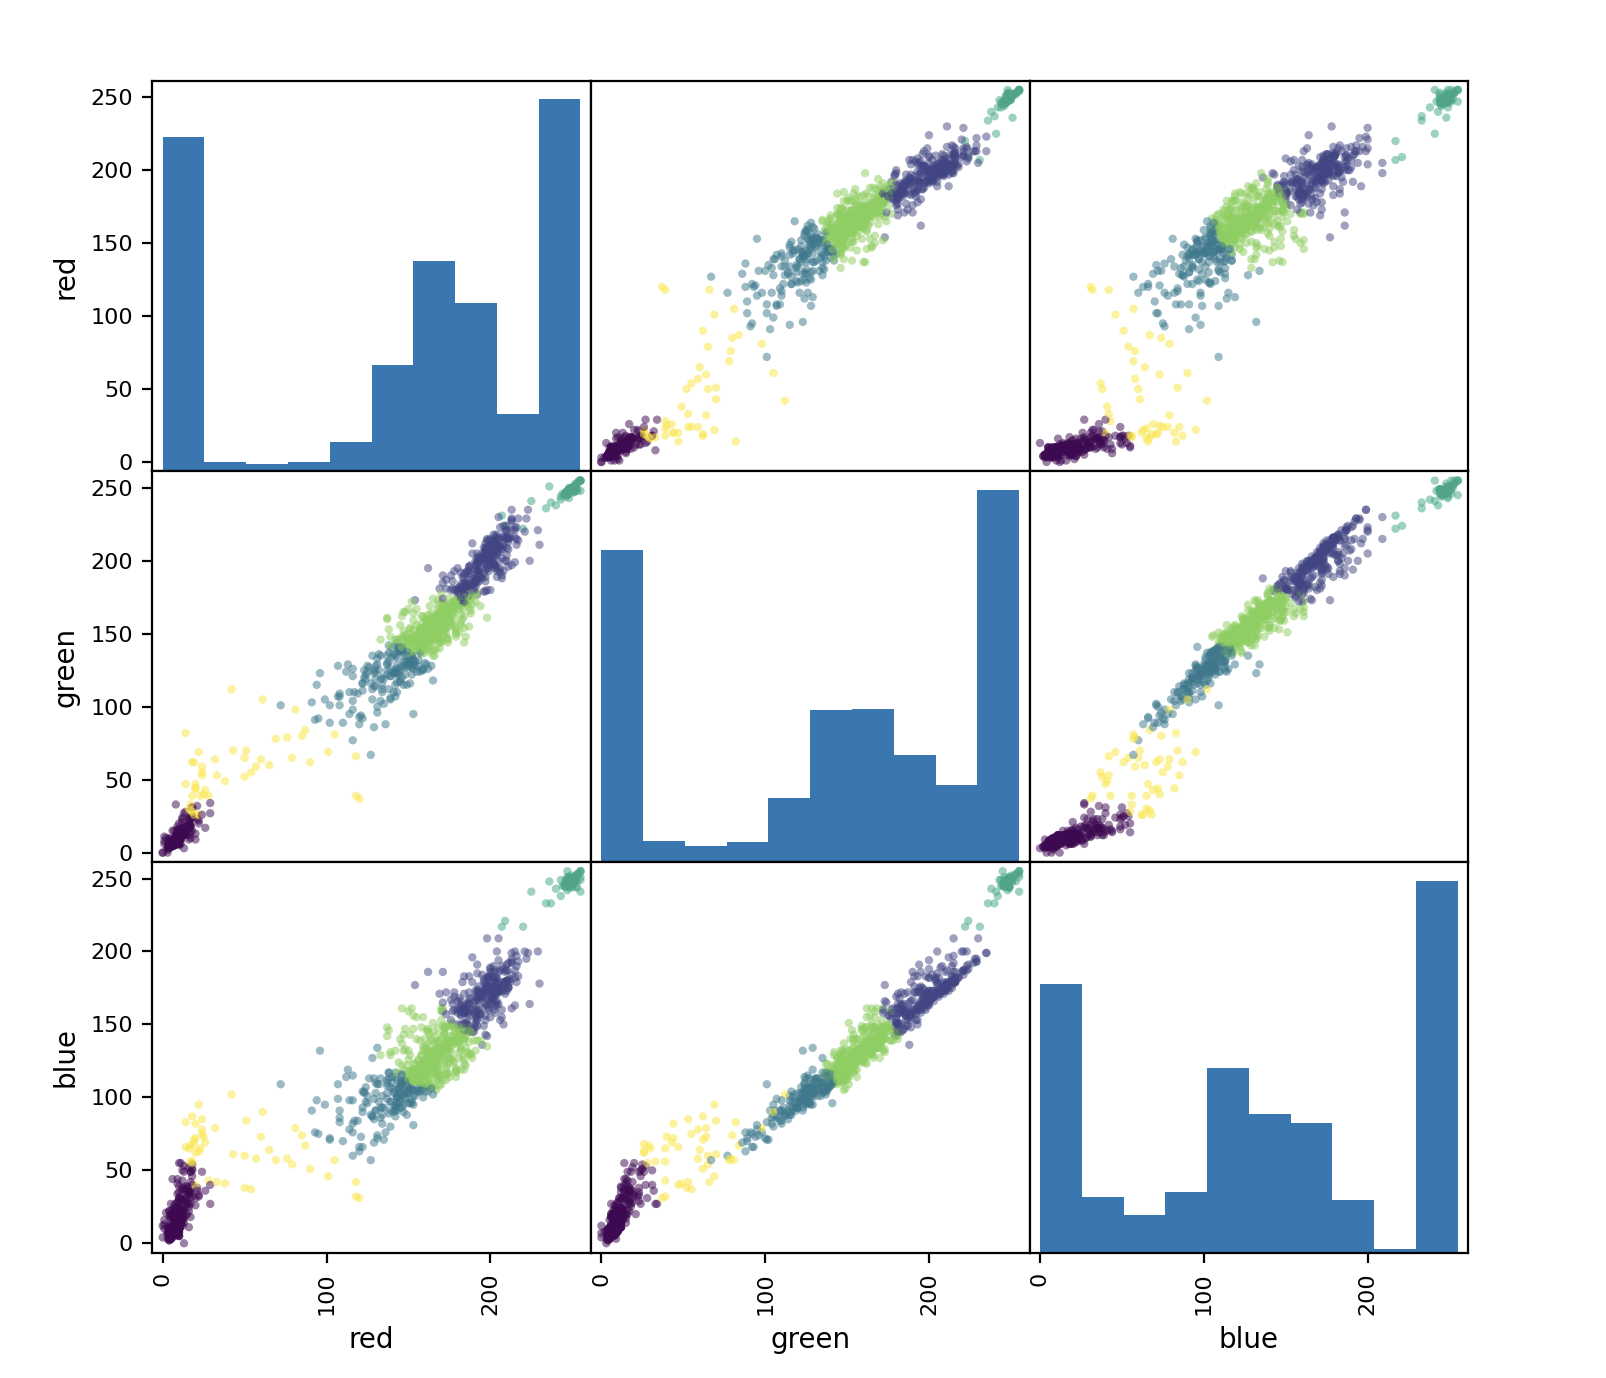
\includegraphics[width=0.75\textwidth]{./img/6.8.1.png}
                \caption{\label{fig:6.4.1}Image 2D}  
            \end{center}
    \end{minipage}\hfill
    \begin{minipage}{.48\linewidth}
        \begin{center}
            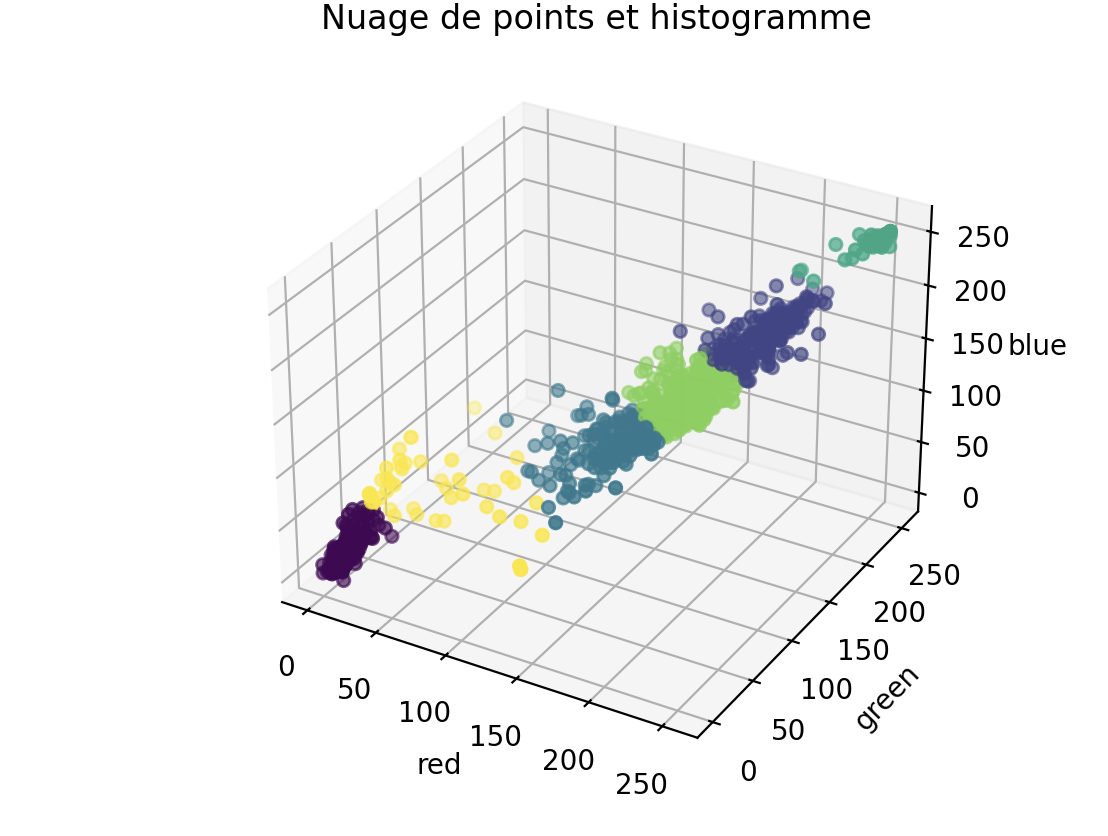
\includegraphics[width=0.75\textwidth]{./img/6.8.2.png}
            \caption{\label{fig:6.4.2}Image 3D}  
        \end{center}
    \end{minipage}
\end{figure}

\clearpage

\begin{figure}[!h]
    \begin{minipage}{.48\linewidth}
        \begin{center}
            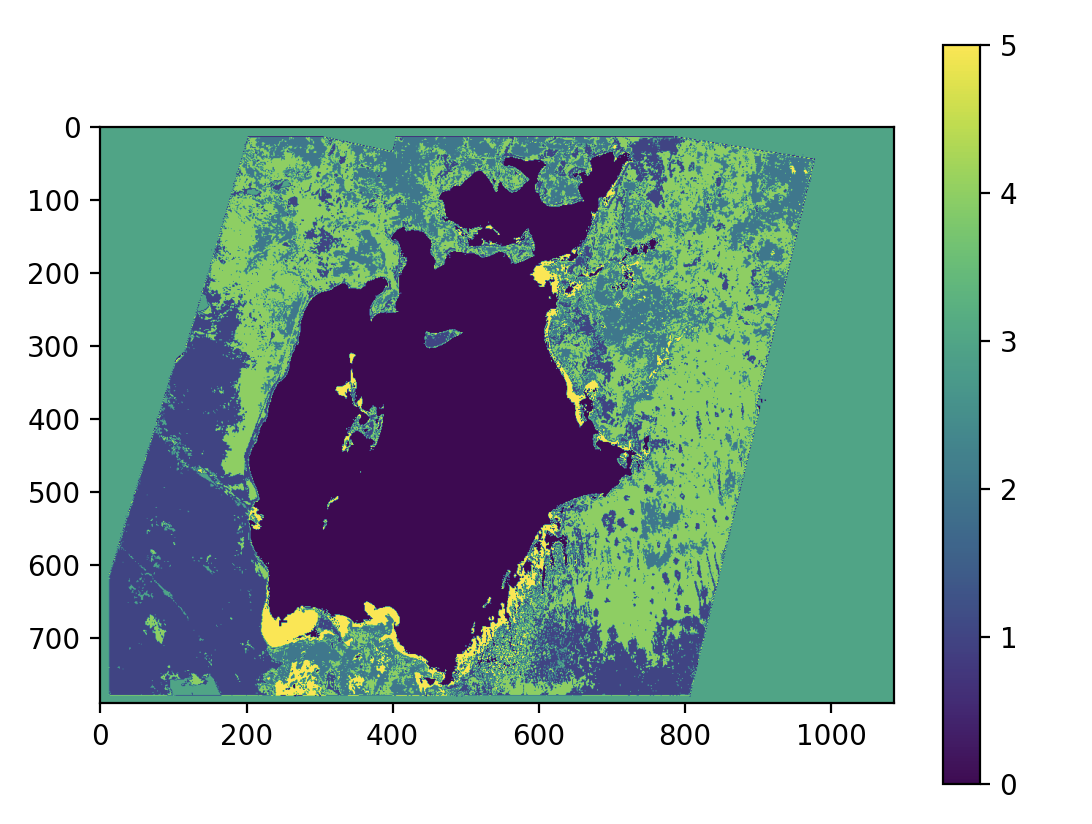
\includegraphics[width=0.75\textwidth]{./img/6.8.3.png}
                \caption{\label{fig:6.4.1}Image 1973 Predicted Labels}  
            \end{center}
    \end{minipage}\hfill
    \begin{minipage}{.48\linewidth}
        \begin{center}
            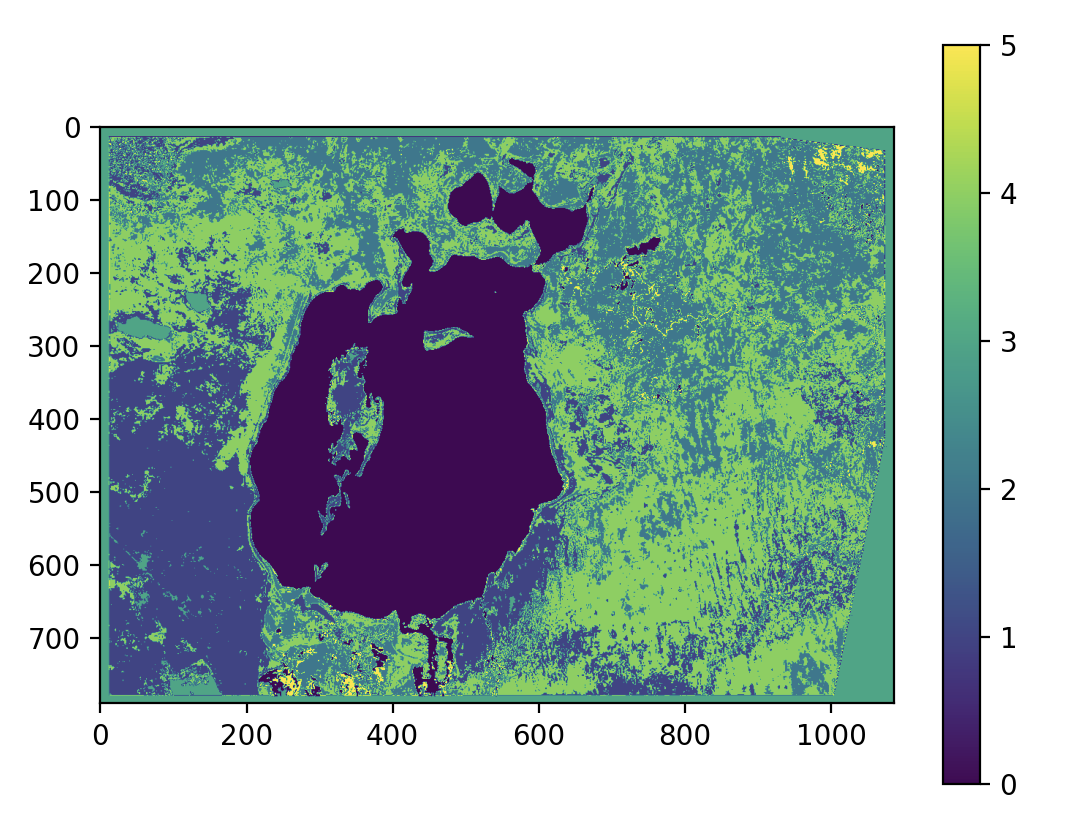
\includegraphics[width=0.75\textwidth]{./img/6.8.4.png}
            \caption{\label{fig:6.4.2}Image 1987 Predicted Labels}  
        \end{center}
    \end{minipage}
\end{figure}

On constate que plus on augmente notre nombre de cluster, moins le pourcentage du niveau de la mer est important. 
Il faut correctement choisir le nombre de cluster pour pas que la mer se retrouve divisé. L’avantage de 3 cluster est 
qu’il détecte bien la mer comme on peut le voir sur les différents graphique. Un chute de 6\% 
du niveau de la mer entre 1973 et 1987 semble cohérent.






















  








